\documentclass{beamer}
\usepackage[utf8]{inputenc}
\usepackage[russian]{babel}
\usepackage{amsmath, amsfonts, amssymb, amsthm, amscd}
\usepackage{graphicx, epsfig, subfig, epstopdf}
\usepackage{longtable}
\usepackage{hyperref}
\usepackage{xypic}

\setbeamertemplate{enumerate items}[circle]
\beamertemplatenavigationsymbolsempty
\usepackage{amsthm}
\newtheorem{thrm}{Теорема}

% notation
\newcommand{\bs}[1] {\boldsymbol #1}
\newcommand{\KL}{\text{KL}}
\newcommand{\Dkl}[1]{D_{\KL}\bigl(#1\bigr)}
\newcommand{\Gen}{\text{\tiny{G}}}
\newcommand{\mst}{m^{*}} % optimal sample size
%\newcommand{\G}{\text{\tiny{G}}} % Doubles Gen
\newcommand{\D}{\text{\tiny{D}}}
\newcommand{\Dnu}{D_{\bs{\nu}}}
\newcommand{\y}{\mathbf{y}}
\newcommand{\x}{\mathbf{x}}
\newcommand{\Y}{\mathbf{Y}} % target matrix
\newcommand{\X}{\mathbf{X}} % data matrix
\newcommand{\Z}{\mathbf{Z}} % data matrix
\newcommand{\z}{\mathbf{z}}
\newcommand{\w}{\mathbf{w}}
\newcommand{\bW}{\mathbf{W}}
\newcommand{\bu}{\mathbf{u}}
\newcommand{\bv}{\mathbf{v}}
\newcommand{\clH}{\bar{H}}
\newcommand\ci{\perp\!\!\!\perp} % conditional independance
\newcommand{\argmin}{\mathop{\rm arg\,min}\limits}
\newcommand{\argmax}{\mathop{\rm arg\,max}\limits}
% probabilities and distributions
\newcommand{\Bern}{\text{Bern}}
\newcommand{\Beta}{\text{Beta}}
\newcommand{\Var}{\mathsf{D}}
\newcommand{\Pgen}{\mathbb{P}}
\newcommand{\pgen}{q}
\newcommand{\prior}{p^{*}}
\newcommand{\Prb}[1]{\mathsf{P}\bigl(#1\bigr)} %{\mathsf{P}}
\newcommand{\Exp}{\mathsf{E}}
% matrices
\newcommand{\Tr}{\mathsf{Tr}}
%\newcommand{\det}{\text{det}}
\newcommand{\diag}{\text{diag}}
\newcommand{\hp}{\hat{p}}
\newcommand{\hP}{\hat{P}}
\newcommand{\ncc}{\text{n.c.~}\chi^2} % non-central
\newcommand{\T}{{\text{\tiny\sffamily\upshape\mdseries T}}}
\newcommand{\R}{{\text{\tiny\sffamily\upshape\mdseries T}}} % Doublе!
\newcommand{\ns}{\text{ns}}
\newcommand{\stat}{\text{st}}
\newcommand{\wD}{\mathbf{w}_{\D}}
\newcommand{\wG}{\mathbf{w}_{\Gen}}
\newcommand{\N}{\text{\tiny\textsl{N}}}
%parametric family
\newcommand{\Fam}{\mathcal{F}}
\newcommand{\W}{\mathcal{W}} % possible parameters values
\newcommand{\Ind}[1] {\mathbb{I}\left[#1\right]} % indicator function
\newcommand{\bigO}[1] {\mathcal{O}\left(#1\right)} % big O

\newcommand{\htns}[1] {\hat {\tns #1}}
\newcommand{\Q}[1] {Q_{#1}}
\newcommand{\bA}{\mathbf{A}}
\newcommand{\bB}{\mathbf{B}}
\newcommand{\bC}{\mathbf{C}}
\newcommand{\bD}{\mathbf{D}}
\newcommand{\ba}{\mathbf{a}}
\newcommand{\bb}{\mathbf{b}}
\newcommand{\bc}{\mathbf{c}}
\newcommand{\bS}{\mathbf{S}}
\newcommand{\bQ}{\mathbf{Q}}
\newcommand{\bU}{\mathbf{U}}
\newcommand{\bfs}{\mathbf{s}}
\newcommand{\bchi}{\boldsymbol{\chi}}
\newcommand{\Nch}{N_{\text{ch}}}
\newcommand{\tmi}[1] {\times_{#1}}
\newcommand{\vc}{\text{vec}}
\newcommand{\corr}{\text{corr}}
\newcommand{\tns}[1] {\underline {\mathbf #1}} % multi-way matrix


% notes and highlights
%\newcommand{\note}[1]{\textcolor{red}{#1}}
\newcommand{\hlmath}[1]{%
  \colorbox{yellow}{$\displaystyle#1$}}
\newcommand{\hl}[1]{\colorbox{yellow}{#1}}%{\textcolor{red}{#1}}
% colors
\definecolor{bluee}{rgb}{0,0,1}
\definecolor{redd}{rgb}{1,0,0}

\setbeamertemplate{footline}[frame number]

\renewcommand{\thefootnote}{\fnsymbol{footnote}}

\newcommand\Wider[2][3em]{%
\makebox[\linewidth][c]{%
  \begin{minipage}{\dimexpr\textwidth+#1\relax}
  \raggedright#2
  \end{minipage}%
  }%
}

\renewcommand{\theorem}{\thefigure.\arabic{subfigure}}

\usepackage{array}
\newcolumntype{M}[1]{>{\centering\arraybackslash}m{#1}}

\renewcommand{\thesubfigure}{\thefigure.\arabic{subfigure}}

\graphicspath{ {./fig/} }


\definecolor{bluee}{rgb}{0,0,1}
\definecolor{redd}{rgb}{1,0,0}
\definecolor{greenn}{rgb}{0,0.7,0}
\definecolor{grey}{rgb}{0.2, 0.2, 0.2}


\DeclareMathOperator*{\inff}{inf}
\newcommand{\Imatr}{I}
\newcommand{\Jmatr}{\mathbf{H}}

%-----------------------------------------------------------------------------------------------------
\title[\hbox to 56mm{ \hfill\insertframenumber\,/\,\inserttotalframenumber}]{Сферические гармоники для моделирования квазипериодических временных рядов}
\author{Тихонов Денис Максимович}
\institute{Московский физико-технический институт\\
Факультет управления и прикладной математики\\
Кафедра интеллектуальных систем}
\date{2021 г.}

%-----------------------------------------------------------------------------------------------------
\begin{document}
\begin{frame}
\maketitle
\end{frame}
%-----------------------------------------------------------------------------------------------------
\begin{frame}{Сферические гармоники для моделирования квазипериодических временных рядов}
\Wider[1em]{\footnotesize
\textbf{Цель работы.} Построение модели аппроксимации квазипериодического временного ряда в фазовом пространстве с использованием сферических гармоник.

\medskip
\textbf{Проблема.} При анализе квазипериодических временных рядов возникает необходимость построения устойчивой модели фазовой траектории в декартовых или сферическом координатах.

Изменяющиеся характерные частоты и амплитуды сигналов приводят к неустойчивости оценок параметров моделей.

\medskip
\textbf{Требуется:}
\begin{enumerate}
    \item предложить способ понижения размерности фазового пространства;
    \item разработать метод аппроксимации устойчивый к шумам, изменению частоты и амплитуды сигнала;
    \item предложить метод отыскания фазы сигнала.
\end{enumerate}
}
\end{frame}
%-----------------------------------------------------------------------------------------------------
\begin{frame}{Литература}

\Wider[3em]{
\footnotesize

\begin{enumerate}
    \item Усманова К. Р. и др. (2020) \textbf{Аппроксимация фазовой траектории квазипериодических сигналов методом сферической регрессии} //\emph{Вестник Московского университета. Серия 15: Вычислительная математика и кибернетика}
    \item \textbf{Aвтоэнкодер для определения фазы сигнала}
    
    Jatesiktat P., Ang W. T. (2017). Unsupervised Phase Extraction Using Dual Autoencoder. // \emph{2017 International Conference on Advanced Computing and Applications}
    \item \textbf{Обнаружение периодов для сегментации биомедицинских сигналов}
    
    Motrenko A., Strijov V. (2015) Extracting fundamental periods to segment biomedical signals //\emph{IEEE journal of biomedical and health informatics}
    \item \textbf{Сферические гармоники для параметризации поверхности сферы}
    
    Nortje С., Ward W., Neuman B., Li Bai, (2015) Spherical Harmonics for Surface Parametrisation and Remeshing // \emph{Mathematical Problems in Engineering}
\end{enumerate}
}
\end{frame}
%-----------------------------------------------------------------------------------------------------
\begin{frame}{Задача аппроксимации фазовой траектории}
\Wider[4em]{
\footnotesize
\begin{columns}
    \column{0.5\textwidth}
    % Временной ряд $\{s_t\}_{t=1}^N$\, назовем \textcolor[rgb]{0.00,0.50,0.00}{квазипериодическим} с периодом $T$, если для всех $t\in[0,+\infty)\,$ найдется $\delta$, такое что для любого $l \in \mathbb{N},$ выполнено
    % $s_{t} \approx s_{t + lT + \delta}, \quad |\delta| \ll T.$
    
    \medskip
    \textbf{Задачи:} $ t \mapsto \mathbf{x} \mapsto \mathbb{H}_{s}^{n} \xrightarrow{} \mathbb{H}_{x}^{p} \xrightarrow{} \mathbb{S}_z^{p} \hookrightarrow [0,2\pi)$
    
    $\mathbb{H}_{s}^{n}$~--- исходное фазовое пространство;
    
    $\mathbb{H}_{x}^{p}$~--- фазовое подпространство в декартовых координатах;
    
    $\mathbb{S}_{z}^{p}$~--- фазовое подпространство в сферических координатах.
    
    \medskip
    Требуется построить:
    \begin{enumerate}
        \item модель $g(\cdot)$, аппроксимирующую фазовую траекторию
    \[ g: \mathbb{R}^{q_1} \times \mathbf{A} \xrightarrow{} \mathbb{S}_{z}^{p},\]
    
        \item модель $f(\cdot)$, восстанавливаюую фазу сигнала
    \[ f: \mathbb{R}^{q_2} \times \mathbb{S}_{z}^{p} \xrightarrow{} [0,2\pi),\]
    
    где $q_1,q_2$ - число параметров модели, $\mathbf{A} = [0,\pi]\times[0,2\pi)\times \dots \times [0,2\pi)$.
    \end{enumerate}
    
    \column{0.3\textwidth}
        \centering
        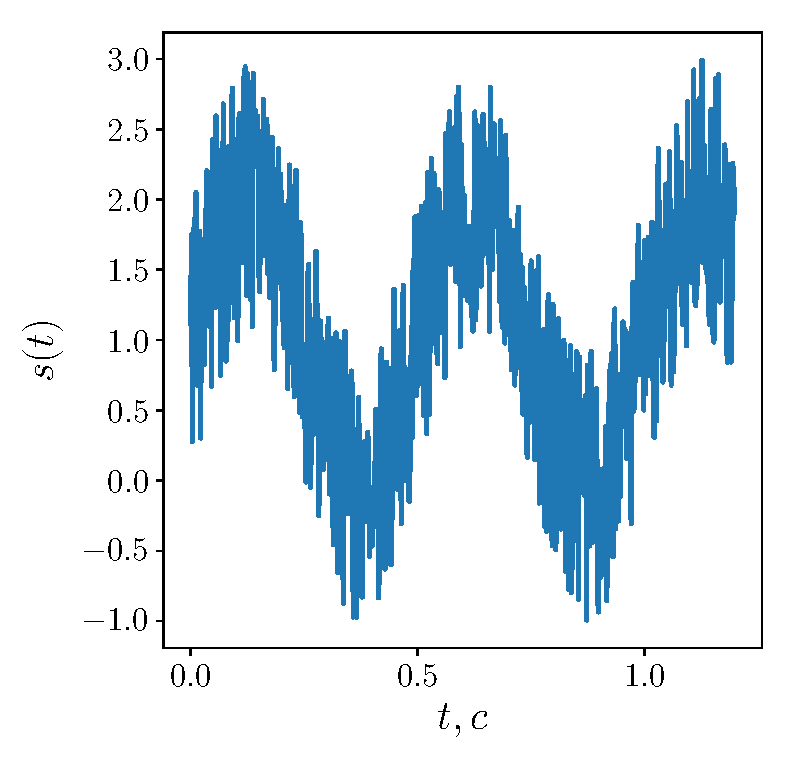
\includegraphics[width=0.7\textwidth]{figs/synthetic_example.eps}
        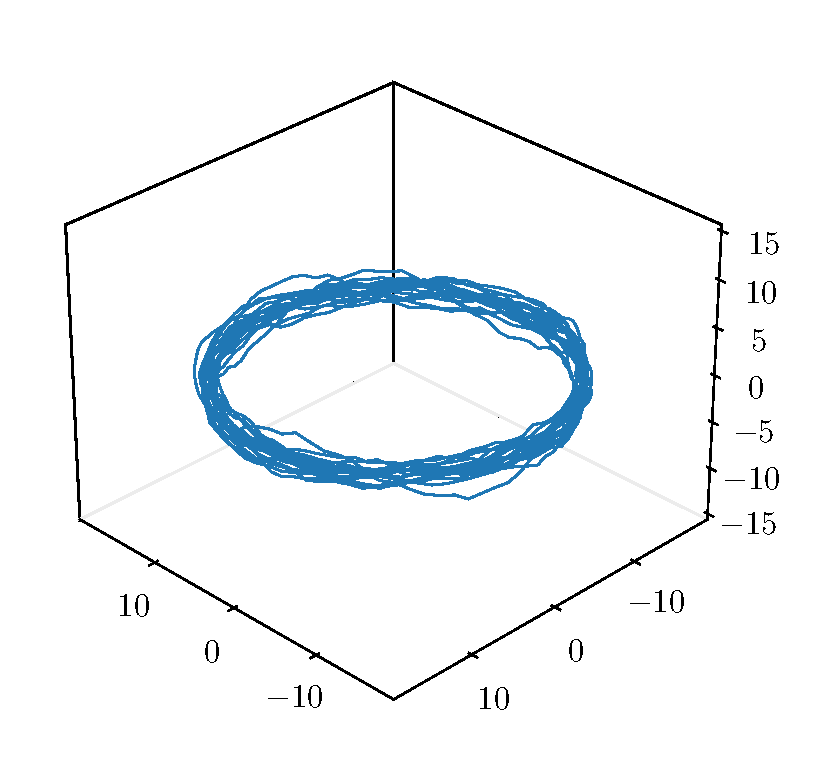
\includegraphics[width=0.8\textwidth]{figs/synthetic_trajectory.eps}
        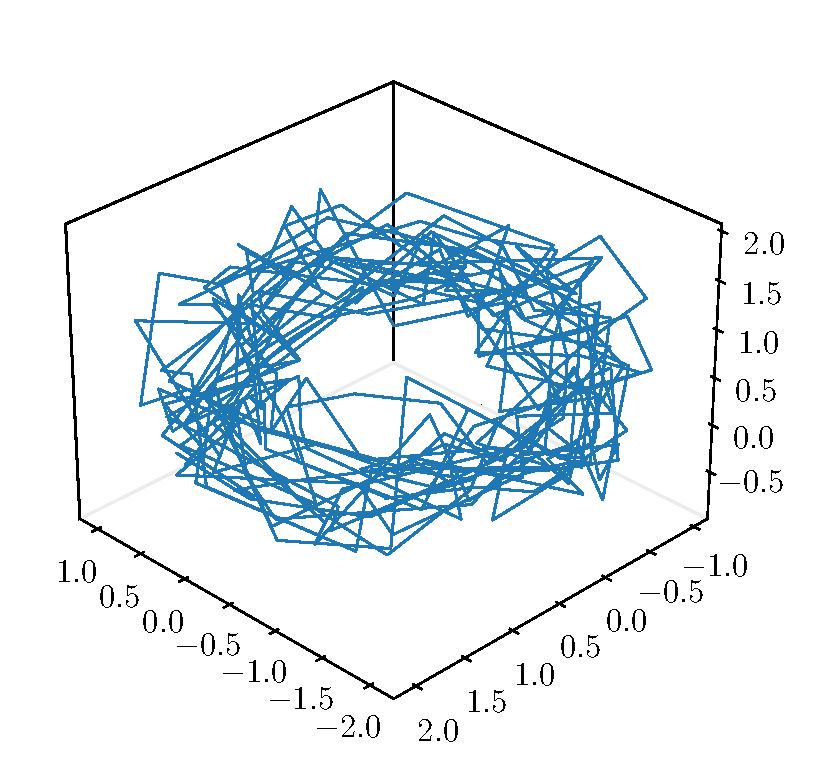
\includegraphics[width=0.8\textwidth]{figs/synthetic_trajectory_nonpca.eps}
\end{columns}

}
\end{frame}
%-----------------------------------------------------------------------------------------------------
\begin{frame}{Методы построения фазового пространства}
\Wider[4em]{
\footnotesize
\begin{columns}
    \column{0.5\textwidth}
    \begin{enumerate}
        \item Метод задержек для построения фазовой траектории
        \[\mathbf{S} = 
        \begin{bmatrix} 
        	s_{1} & \ldots & s_{n}\\
        	s_{2} & \ldots & s_{n+1}\\
        	\vdots& \ddots & \vdots\\
        	s_{N-n+1}&\ldots &s_{N}\\
        \end{bmatrix} =
        	\begin{bmatrix} 
              	\mathbf{s}_{1}\\
              	\mathbf{s}_{2}\\
              	\vdots\\
              	\mathbf{s}_{N-n+1}\\
           \end{bmatrix},
           \quad
           \mathbf{s}_{i} \in \mathbb{H}_{s}^{n}
           \]
        где $n$~--- ширина окна;
        \item Метод PCA для построения фазового подпространства меньшей размерности $p \ll n$.
        \[\mathbf{X} = \mathbf{S W} =
            \begin{bmatrix}
                \mathbf{x}_1 \\
                \mathbf{x}_2  \\
                \dots \\
                \mathbf{x}_{N-n+1}
            \end{bmatrix},
            \quad
            \mathbf{x}_{i} \in \mathbb{H}_{p}^{x},\]
            где $\mathbf{W}$ --- матрица вращения.
            \end{enumerate}
    \column{0.3\textwidth}
            \centering
            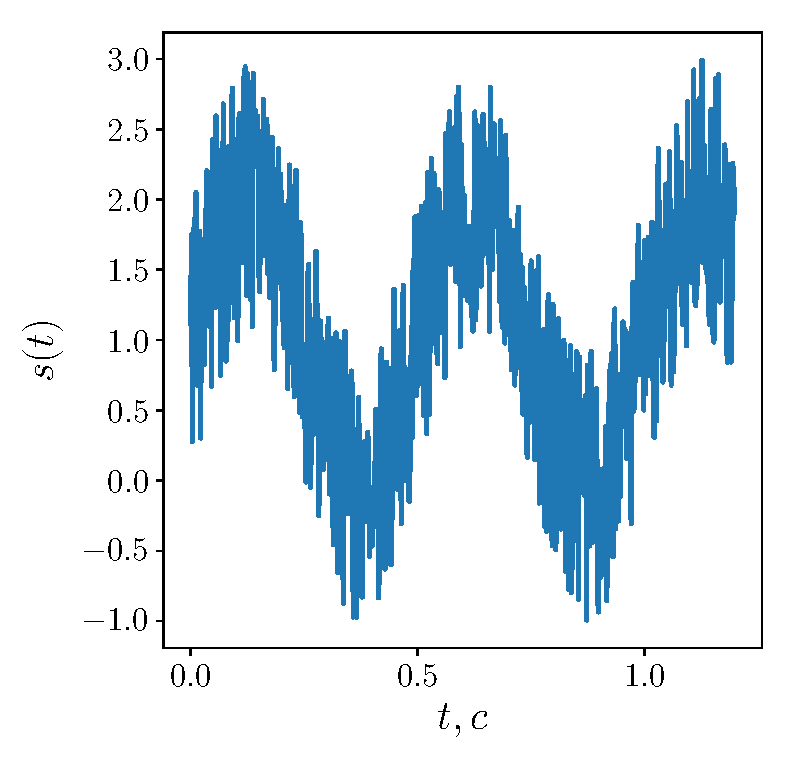
\includegraphics[width=0.7\textwidth]{figs/synthetic_example.eps}
            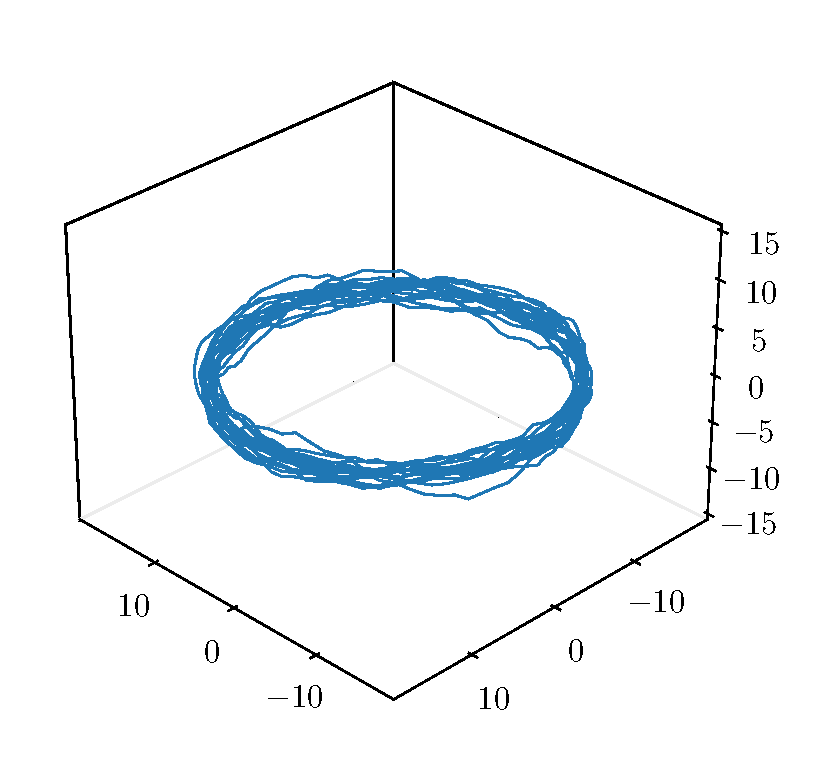
\includegraphics[width=0.8\textwidth]{figs/synthetic_trajectory.eps}
            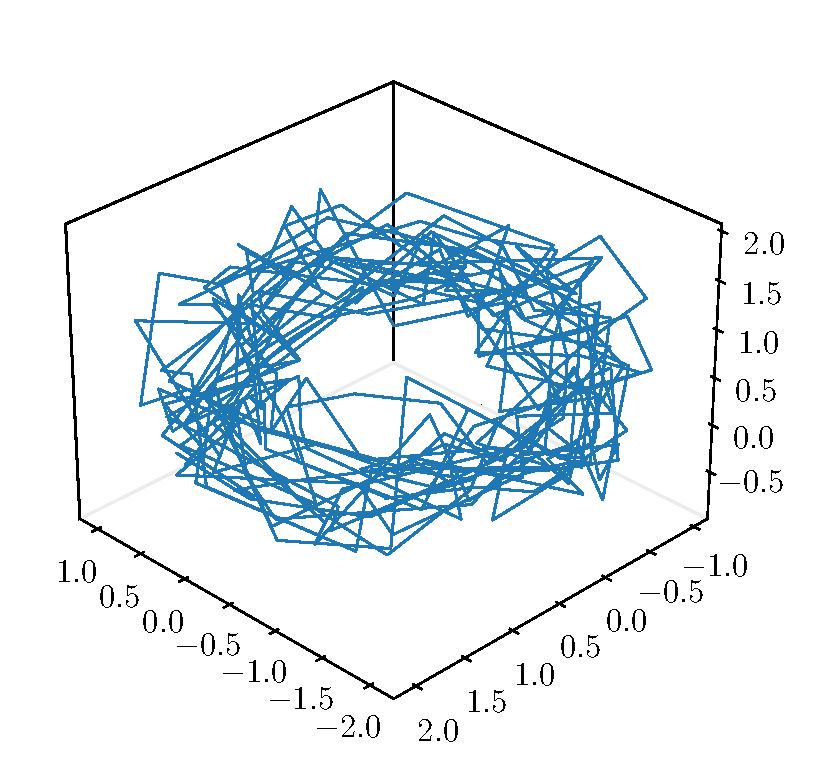
\includegraphics[width=0.8\textwidth]{figs/synthetic_trajectory_nonpca.eps}
\end{columns}
}
\end{frame}
%-----------------------------------------------------------------------------------------------------
\begin{frame}{Сферическое представление фазовой траектории}

\Wider[3em]{
\footnotesize
\begin{columns}
    \column{0.01\textwidth}
    \column{0.6\textwidth}
        \begin{enumerate}
            \item Предполагается, что структура модели проще в сферических координатах.
            \item В полученном подпространстве $\mathbb{X} \subseteq \mathbb{R}^{p}$ строится отображение из декартовых координат в сферические:
            \[\phi: \mathbf{x} \xrightarrow{} \mathbf{z} = [r,\alpha_{p-1},\dots,\alpha_1],
            \quad
            \mathbf{a} = [\alpha_{p-1},\dots,\alpha_1]\].
            
            \item Точки $\mathbf{a}$ задают функцию ${f_{\text{real}}}(\mathbf{a}(t)) \quad$ $t\in[0,+\infty)$ на поверхности сферы $\mathbb{S}^{p-1}$.
        \end{enumerate}
    \column{0.4\textwidth}
    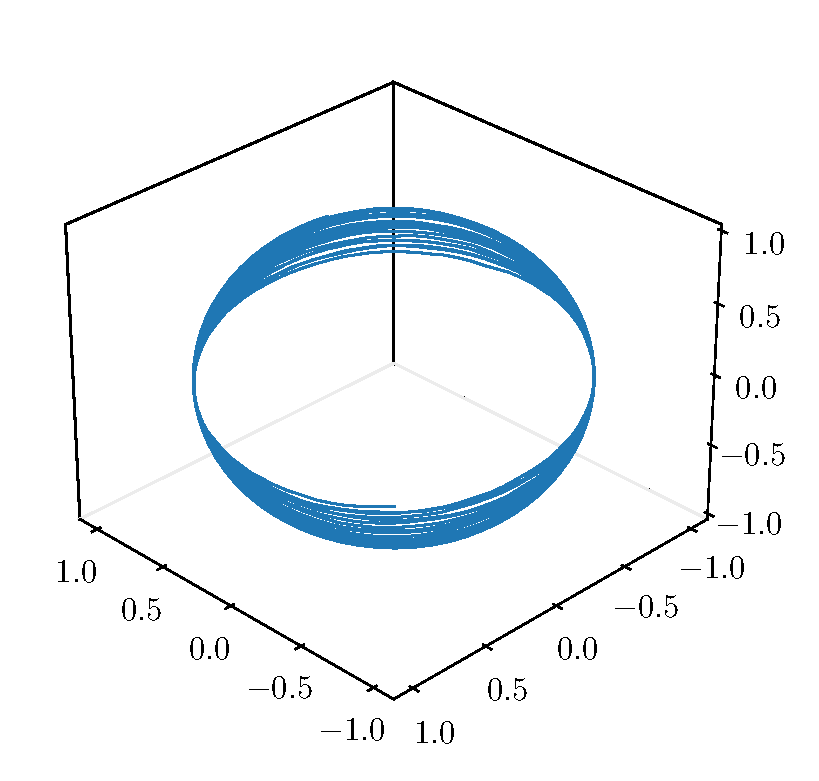
\includegraphics[width=0.85\textwidth]{figs/synthetic_trajectory_r1.eps}
    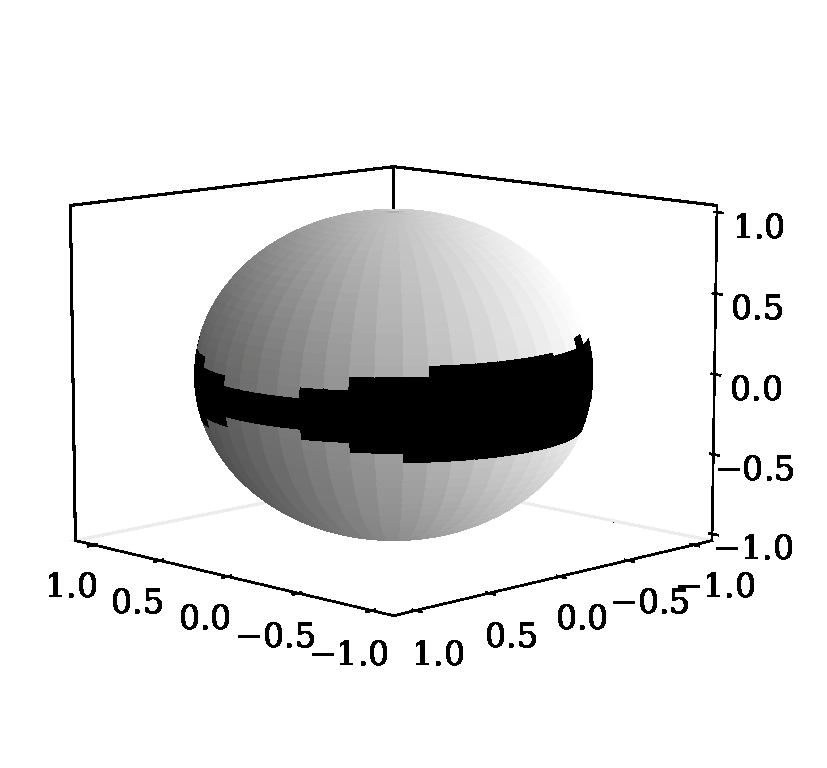
\includegraphics[width=0.85\textwidth]{figs/synthetic_trajectory_sp_proj.eps}
    \end{columns}
}
\end{frame}
%-----------------------------------------------------------------------------------------------------
\begin{frame}{Аппроксимация сферическими гармониками}

\Wider[6em]{
\footnotesize
\begin{columns}
    \column{0.01\textwidth}
    \column{0.6\textwidth}
        \begin{enumerate}
            \item Предлагается аппроксимировать фазовую траекторию на поверхности сферы с помощью сферических гармоник:
            \[f_{\text{sp}}(\mathbf{w}_{sp},\mathbf{a}) = \sum_{l_{p-1} = 0}^{N_{\text{approx}}}\sum_{l_{p-2} = 0}^{l_{p-1}}...\sum_{l_1 = -l_2}^{l_2}
            w_{l_{p-1},...,l_1} Y_{l_{p-1},...,l_1}(\mathbf{a})\],
            
            \item Базисные функции представимы в виде \[Y_{l_{p-1},...,l_1}(\mathbf{a}) = 
            \left[\prod\limits_{k = 2}^{p-1}{_k}{\overline{P}}_{l_k}^{l_{p-1}}(\alpha_k)\right]
	    \frac{1}{\sqrt{2\pi}}
	    \exp{(i l_1 \alpha_1)}\],
        где $l_{p-1},...,l_1$ - индексы удовлетворяющие
        \[l_{p-1} \geq l_{p-2} \geq \dots \geq l_2 \geq|l_1|.\]
            
            \item Решается задача 
            \[\mathbf{\hat{w}}_{sp} = \argmin_{\mathbf{w}_{sp}}
    \|f_{\text{real}}(\mathbf{a}(t)) - f_{\text{sp}}(\mathbf{w}_{sp},\mathbf{a}(t))\|^2\].
        \end{enumerate}
    \column{0.4\textwidth}
    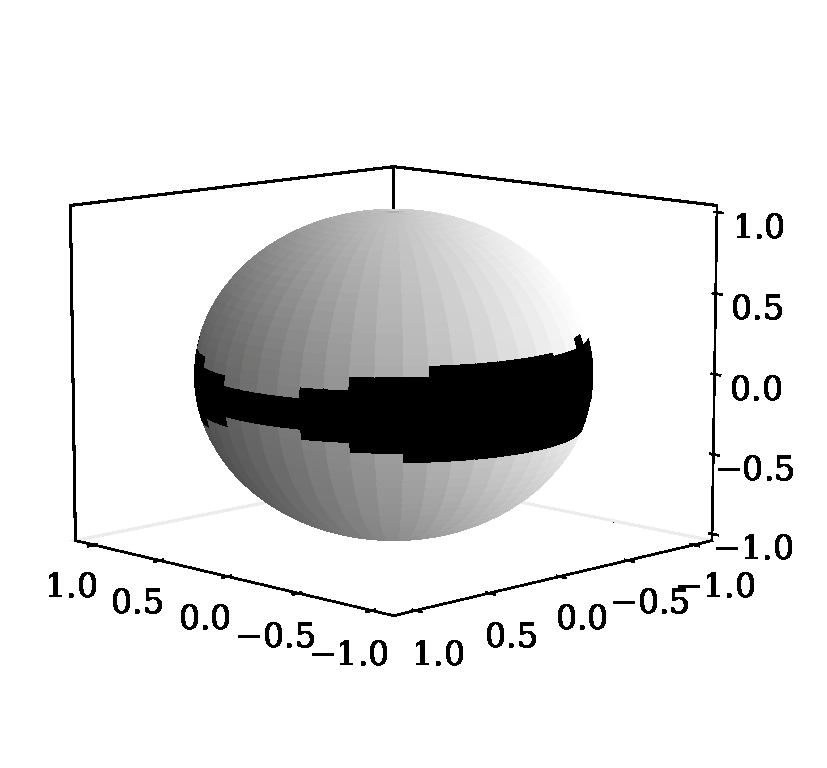
\includegraphics[width=0.85\textwidth]{figs/synthetic_trajectory_sp_proj.eps}
    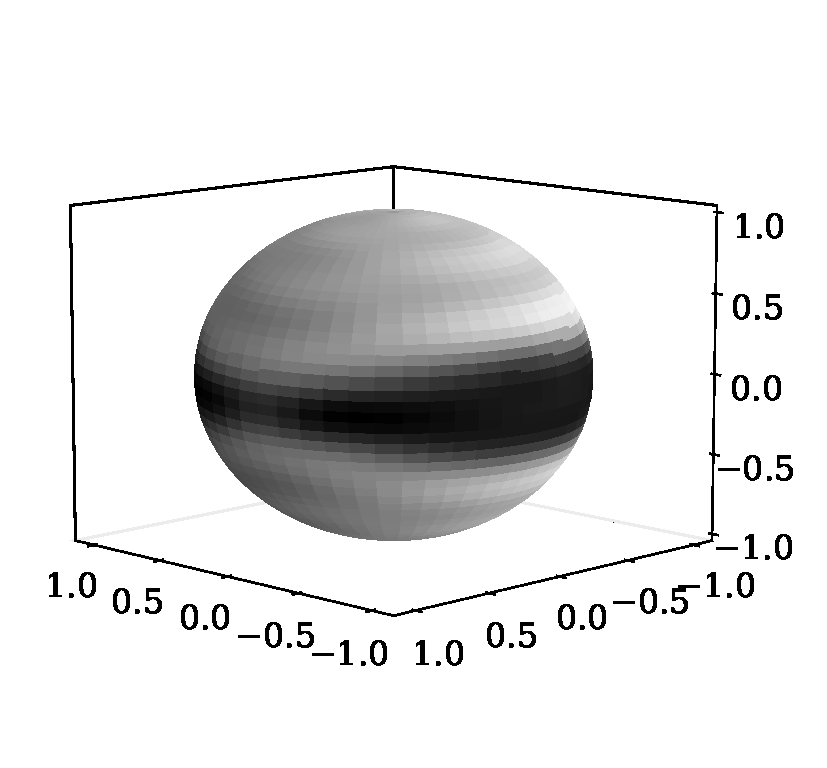
\includegraphics[width=0.85\textwidth]{figs/synthetic_trajectory_sp_harm.eps}
    \end{columns}
}
\end{frame}
%-----------------------------------------------------------------------------------------------------
\begin{frame}{Восстановление фазы сигнала}

\Wider[2em]{
\footnotesize
 Предлагается восстанавливать фазу сигнала с помощью автоэнкодера в фазовом сферическом подпространстве:
\[\phi(t) = \sigma(\mathbf{W}_{\text{enc}}\mathbf{a}(t)
+ \mathbf{b}_{\text{enc}}
),
\quad
\mathbf{\hat{a}}(t) = \sigma(\mathbf{W}_{\text{dec}}\phi(t)
+ \mathbf{b}_{\text{dec}}).\]

С решением в виде  $\mathbf{W}_{\text{enc}} = \argmin\|\mathbf{a}(t) - \mathbf{\hat{a}}(t)\|^2_2 $.

\medskip
\begin{columns}
    \column{0.5\textwidth}
    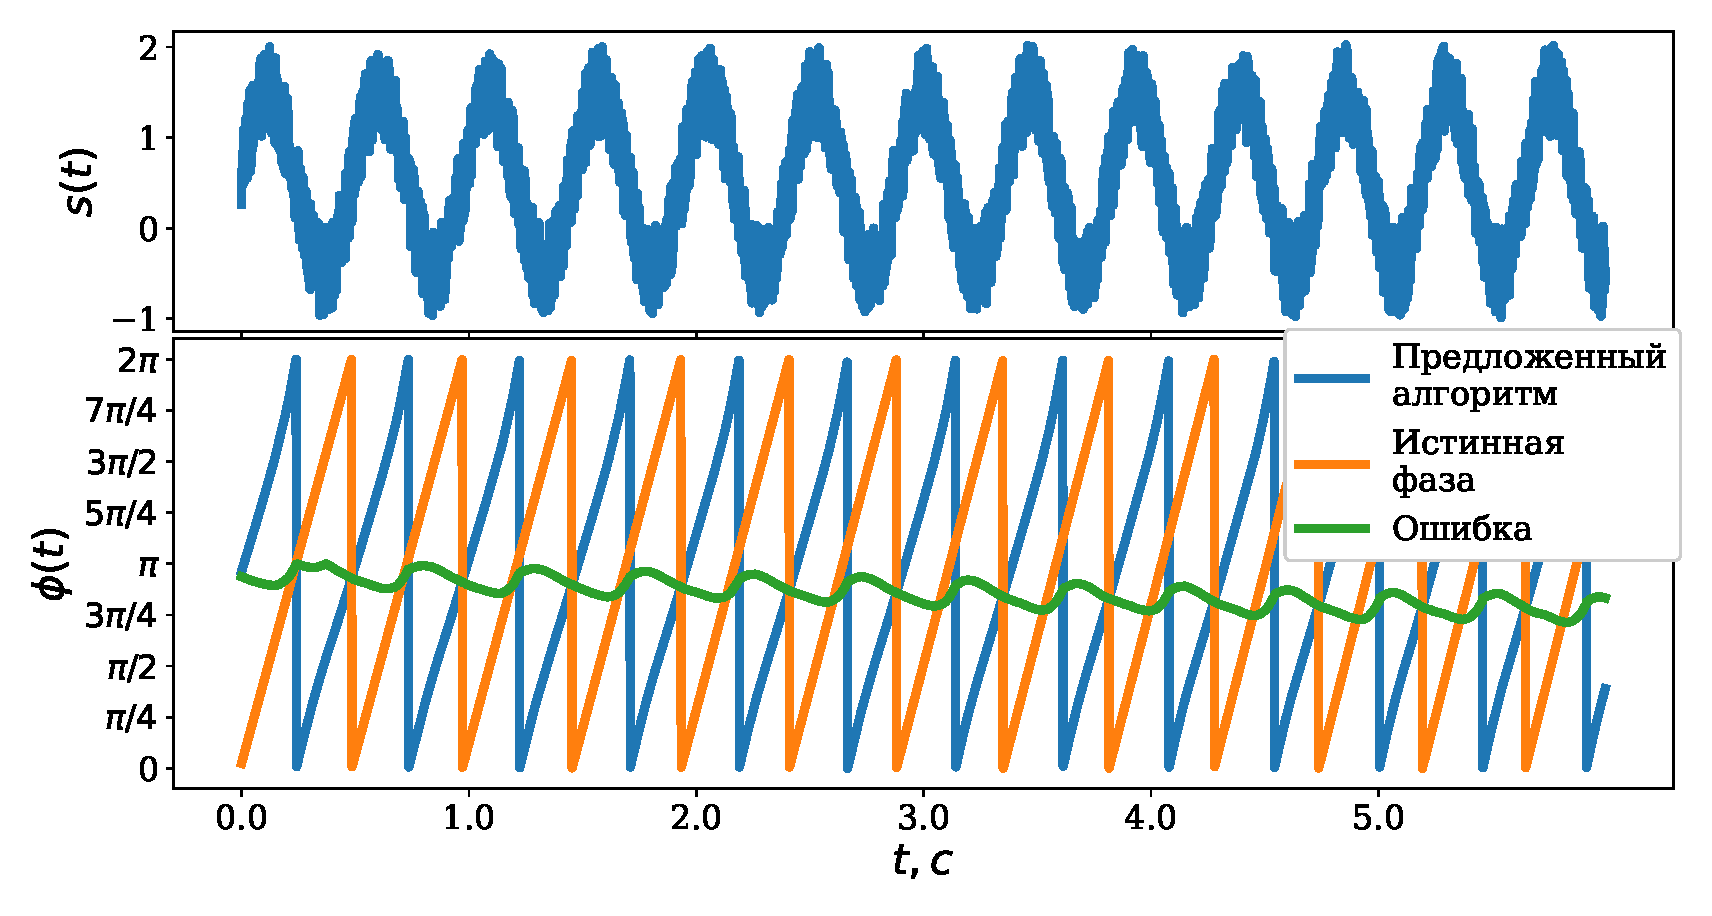
\includegraphics[width=1\textwidth]{figs/synthetic_trajectory_phase.eps}
    \column{0.5\textwidth}
    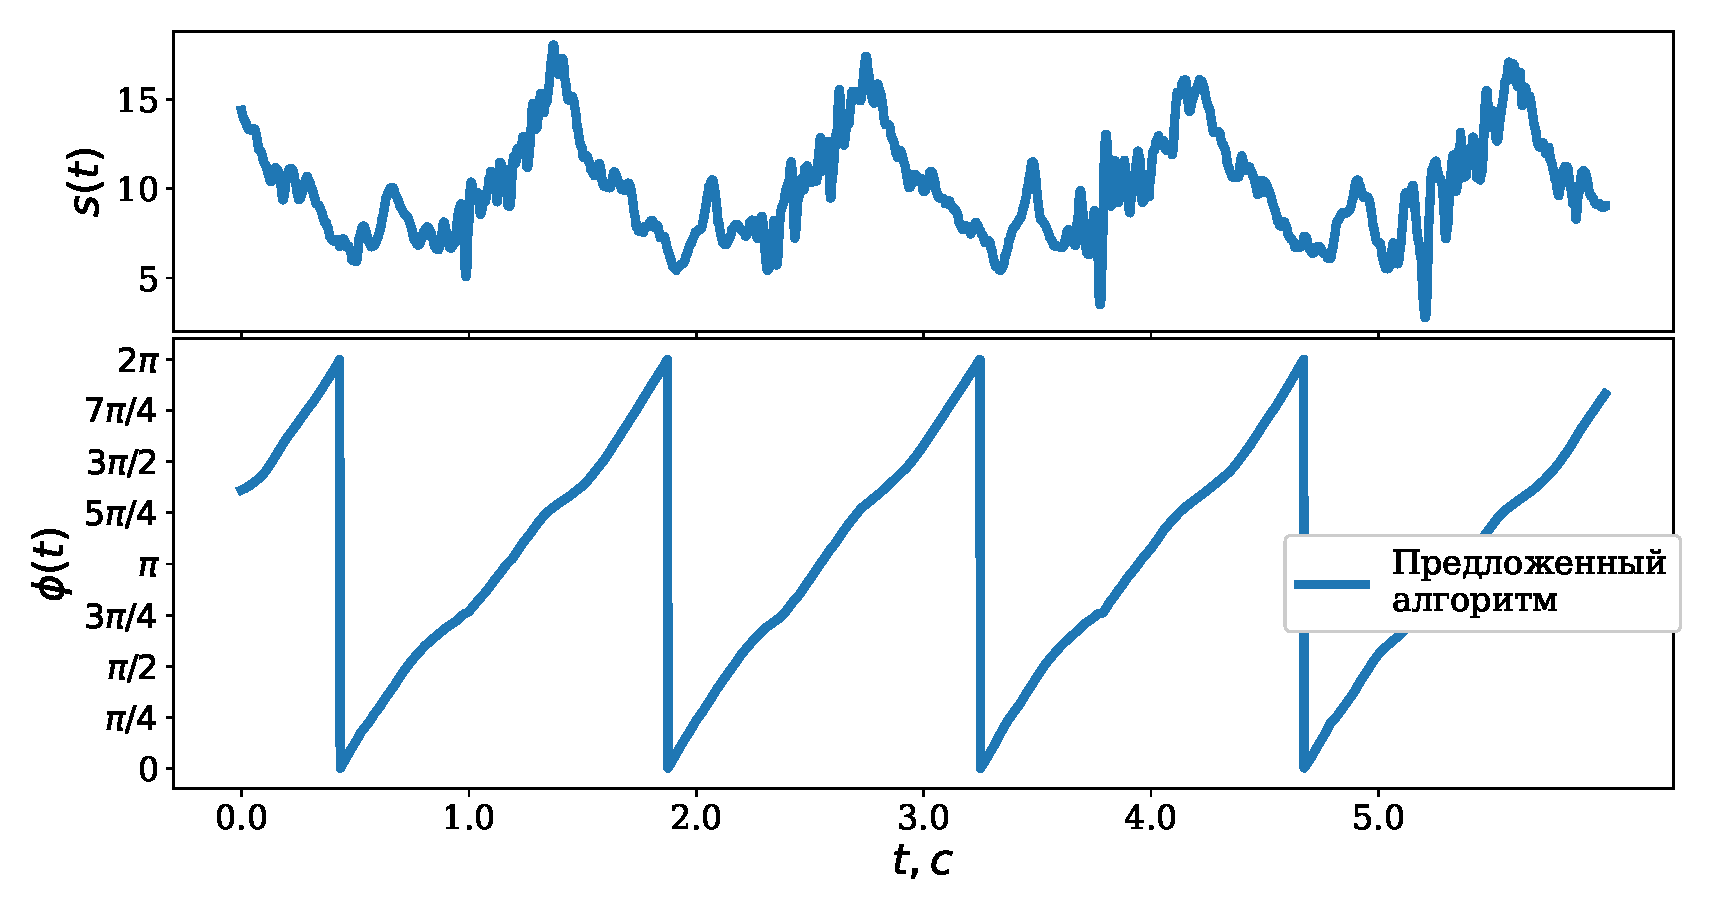
\includegraphics[width=1\textwidth]{figs/real_trajectory_phase.eps}
\end{columns}

}
\end{frame}



%-----------------------------------------------------------------------------------------------------
\begin{frame}{Качество аппроксимации на реальных данных с акселерометра}

\Wider[2em]{
\footnotesize
\centering
\begin{tabular}{p{0.5cm}p{3cm}p{3cm}p{3cm}}
      & Временной ряд
      & Фазовая траектория в 3D
      & Аппроксимация гармониками
      \\
    \hline
    \rotatebox{90}{ \text{Велопрогулка} }
    & 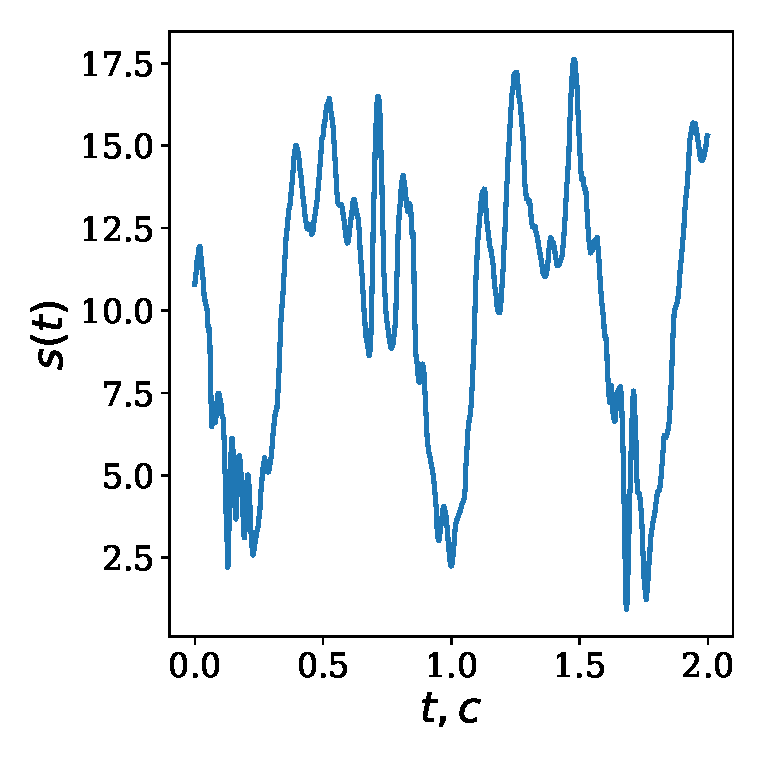
\includegraphics[scale=0.2]{./figs/bike_example.eps}
    & 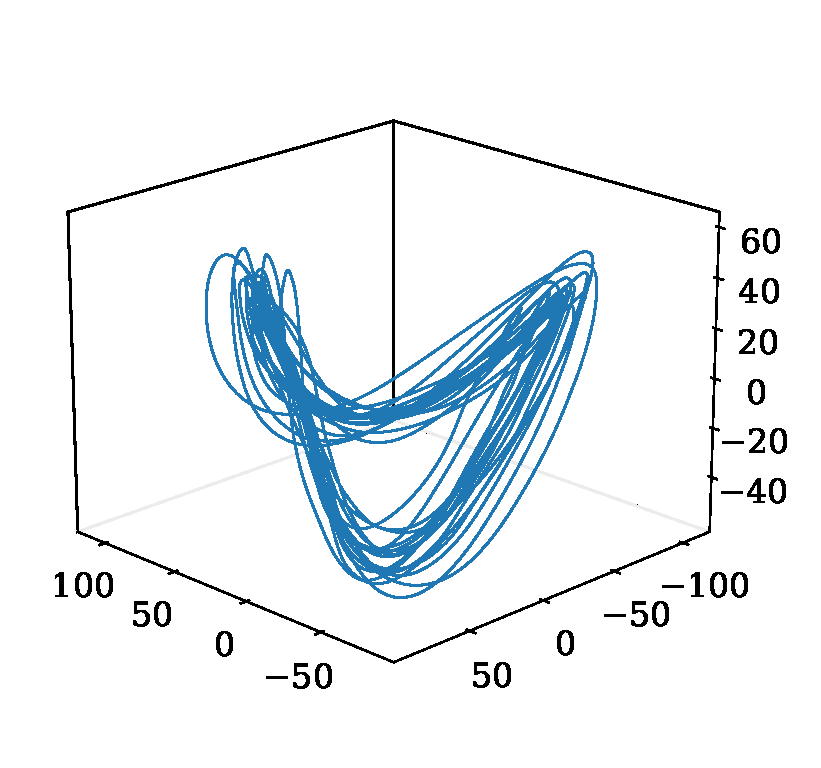
\includegraphics[scale=0.2]{./figs/bike_trajectory.eps}
    & 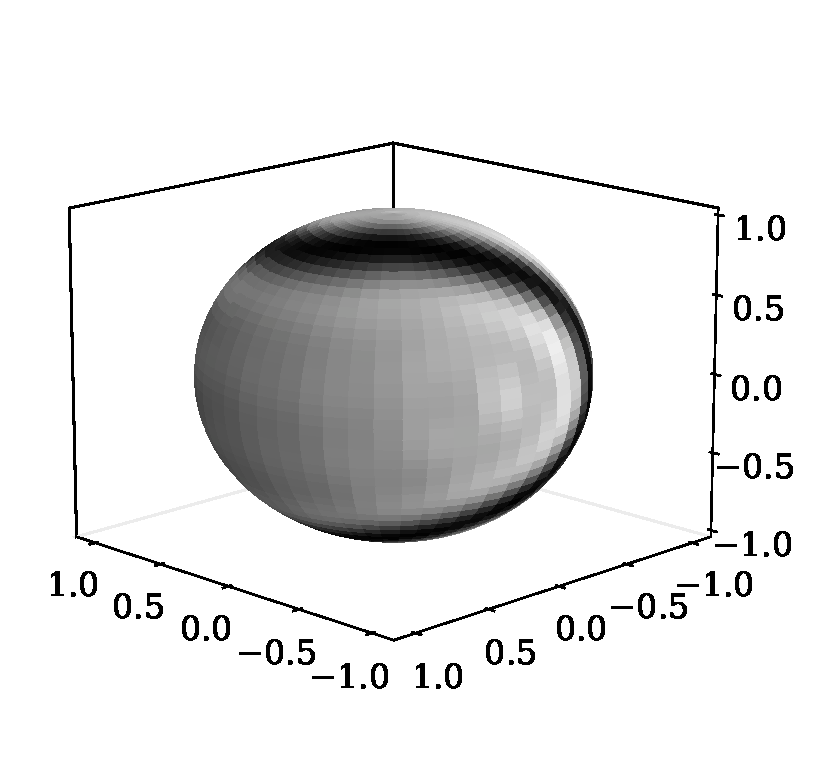
\includegraphics[scale=0.2]{./figs/sph_harm_bike.eps}
    \\ 
    \hline
    
    \rotatebox{90}{ \text{Приседания} }
    & 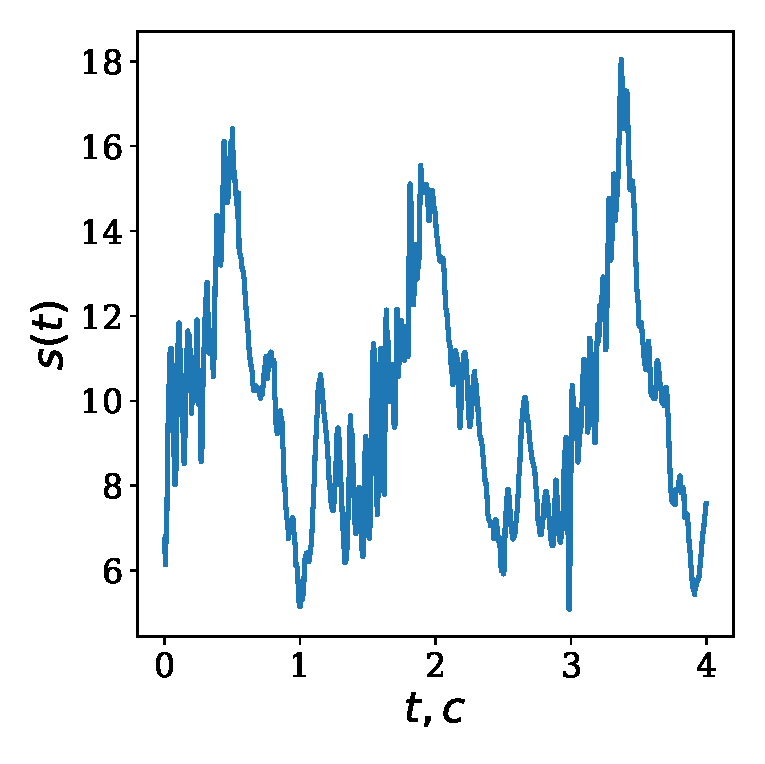
\includegraphics[scale=0.2]{./figs/squats_example.eps}
    & 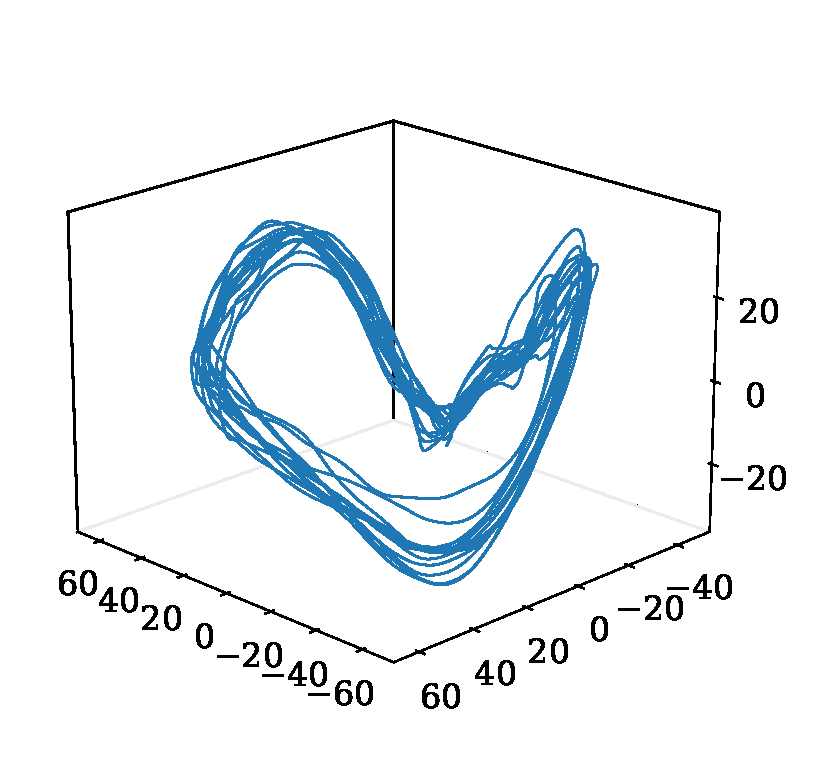
\includegraphics[scale=0.2]{./figs/squats_trajectory.eps}
    & 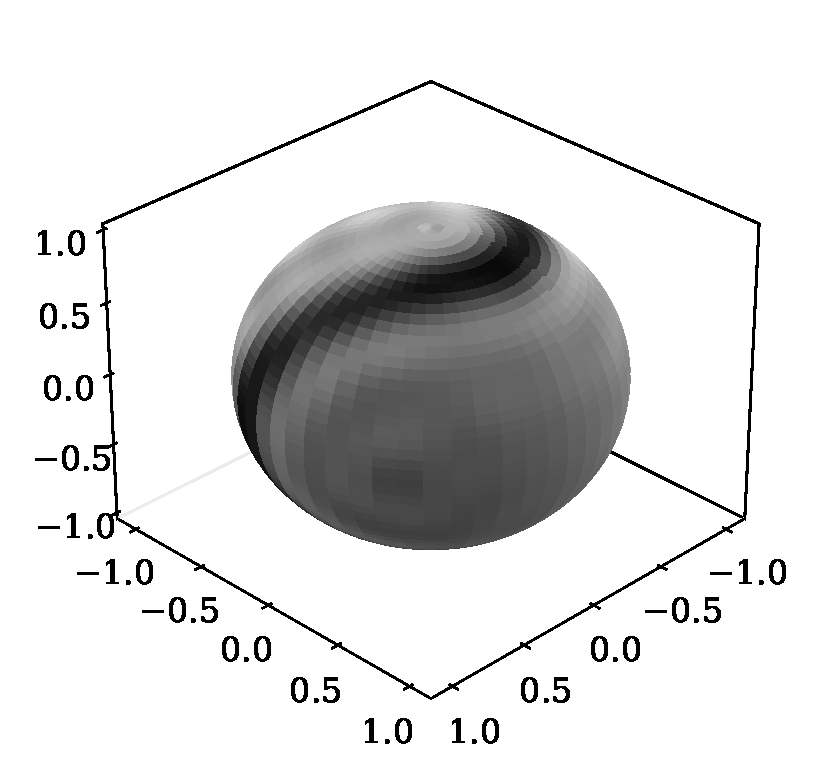
\includegraphics[scale=0.2]{./figs/sph_harm_squats.eps} \\ 
    \hline
\end{tabular}
}
\end{frame}
%-----------------------------------------------------------------------------------------------------
\begin{frame}{Заключение}

\Wider[3em]{
\footnotesize
Предложенная композиция методов позволяет уменьшить количество параметров с нескольких тысяч, в случае с полноценным автоэнкодером, до нескольких сотен.
В частности:
\begin{enumerate}
    \item Предложен метод построения и уменьшения фазового пространства. Метод построении векторов задержек и разложения на главные компоненты;
    \item Предложен метод аппроксимации фазовой траектории в сферических координатах произвольной размерности с использованием сферических гармоник;
    \item Разработан метод восстановления фазы основанный на автоенкодере в пространства углов.
\end{enumerate}
}
\end{frame}
\end{document}
